\sn{On The Rigour of A Random Variable}{
For the beginning of this module, a random variable $X$ is considered to be a function from a sample space $\Omega$ to the unit interval $[0, 1]$. However, in Lectures 6 and 7, we use the full definition of a random variable, which is a measurable function from a sample probability space $(\Omega)$ to a measurable space $(E, \varepsilon)$, involving the concept of $\sigma$-algebras and measure spaces. \bigskip

When the sample space is a continuous space, the function $p$ is a \textbf{probability density function} (PDF). When the sample space is a discrete space, the function $p$ is a \textbf{probability mass function} (PMF).
} 


\marginnote[-60pt]{We will introduce measure theory later.}





\section{Brief Probability Theory Review}

$x$ is a sample from a random variable $X$. 

\noindent $P(X=x)$ refers to probability that the random variable $X$ takes on the value $x$.

\subsection{Probability Density Function (PDF)}
\begin{marginfigure}[100pt]
    \centering
    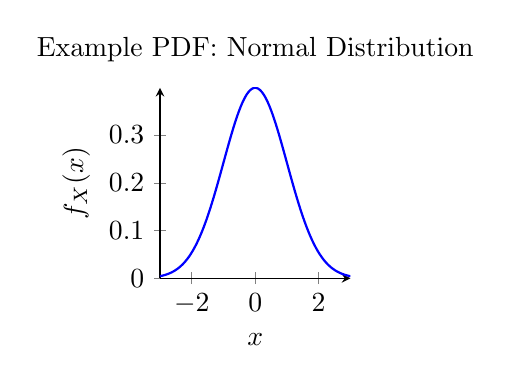
\begin{tikzpicture}
        \begin{axis}[
            width=4cm,
            height=4cm,
            xlabel={$x$},
            ylabel={$f_X(x)$},
            domain=-3:3,
            samples=100,
            axis lines=left,
            ymin=0,
            legend pos=north east,
            title={Example PDF: Normal Distribution}
        ]
        \addplot[blue, thick] {exp(-x^2 / 2) / sqrt(2 * pi)};
        \end{axis}
    \end{tikzpicture}
    \caption{Probability Density Function of a standard normal distribution}
\end{marginfigure}

The Probability Density Function (PDF) of a continuous random variable \(X\) is a function \(f_X(x)\) that describes the relative likelihood for this random variable to take on a given value. The PDF has the following properties:
\begin{itemize}
    \item \(f_X(x) \geq 0\) for all \(x\).
    \item \(\int_{-\infty}^{\infty} f_X(x) \, dx = 1\).
\end{itemize}

Mathematically, the PDF is defined such that the probability that \(X\) lies within a particular interval \([a, b]\) is given by:
\[
P(a \leq X \leq b) = \int_{a}^{b} f_X(x) \, dx.
\]


\subsection{Cumulative Distribution Function (CDF)}
\begin{marginfigure}[50pt]
    \centering
    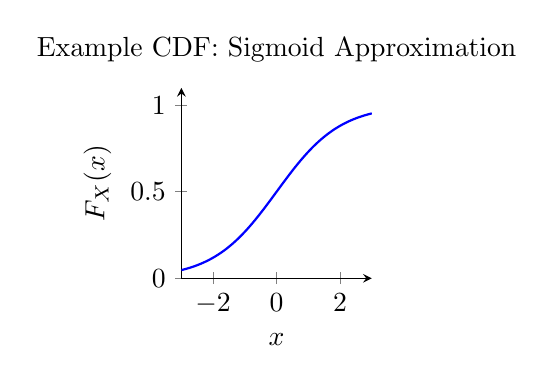
\begin{tikzpicture}
        \begin{axis}[
          width=4cm,
          height=4cm,
            xlabel={$x$},
            ylabel={$F_X(x)$},
            domain=-3:3,
            samples=100,
            axis lines=left,
            ymin=0, ymax=1.1,
            legend pos=south east,
            title={Example CDF: Sigmoid Approximation}
        ]
        \addplot[blue, thick] {1 / (1 + exp(-x))};
        \end{axis}
    \end{tikzpicture}
    \caption{Cumulative Distribution Function}
\end{marginfigure}

The Cumulative Distribution Function (CDF) of a continuous random variable \(X\) is a function \(F_X(x)\) that describes the probability that \(X\) will take a value less than or equal to \(x\). It is defined as:
\[
F_X(x) = P(X \leq x) = \int_{-\infty}^{x} f_X(t) \, dt.
\]

The CDF has the following properties:
\begin{itemize}
    \item \(0 \leq F_X(x) \leq 1\) for all \(x\).
    \item \(F_X(x)\) is a non-decreasing function.
    \item \(\lim_{x \to -\infty} F_X(x) = 0\).
    \item \(\lim_{x \to \infty} F_X(x) = 1\).
\end{itemize}


\subsection{Dealing with Data (Single-Feature)}

In Machine Learning (ML), we often deal with large datasets from which we aim to extract meaningful insights. It is useful to model these data points as random variables:
\[
\{x_1, x_2, \ldots, x_N\}
\]


\noindent We typically model these samples as random variables:

\[
\{x_1 \sim X_1, x_2 \sim X_2, \ldots, x_N \sim X_N\}
\]

\subsection{Vectors of Random Variables}

When dealing with joint random variables, we often represent them as vectors:

\[
\mathbf{X} = (X_1, X_2, X_3) \quad \text{with joint distribution} \quad p_{X_1, X_2, X_3}(x_1, x_2, x_3)
\]

\noindent For a vector of random variables \(\mathbf{X}\) in \( \mathbb{R}^3 \), the joint probability density function is denoted as:

\[
p_{\mathbf{X}}(\mathbf{x}) \quad \text{where} \quad \mathbf{X} \in \mathbb{R}^3
\]
\noindent 
If these are input observations, they are often referred to as "feature vectors."

\subsection{Distinct Random Variables}

We model samples as distinct random variables \sidenote[][-20pt]{\textbf{Why should we model these as distinct random variables? Aren't they all the same thing?} \smallskip

\noindent Despite being identically distributed, distinct random variables allow for capturing dependencies and interactions between different samples.
}:\bigskip

\[
\{x_1 \sim X_1, x_2 \sim X_2, \ldots, x_N \sim X_N\}
\]


\section{Independent and Identically Distributed (i.i.d.) Random Variables}

\marginnote[-50pt]{    \textbf{Why do we model samples as distinct random variables?}

\begin{enumerate}
    \item By treating each sample as a distinct variable, we assume samples are i.i.d, allowing every sample to contribute independently to the likelihood of oberving the data given the model prarameters – so every sample provides unique information to estimate the parameters of the underlying distribution. If we treated all samples as a single random variable, we would lose the granularity of information, leading to a poorer estimate.
    \item Treating samples as distinct allows us to study and model the relationships and dependencies between them.
    \item The assumption of i.i.d follows many results in probability and statistics, such as the Central Limit Theorem, which states that the sum of a large number of i.i.d. random variables is approximately normally distributed. It is also an assumed requirement for a model to generalise. The assumption simplifies the analysis and derivation process, allowing us to use techniques like maximum likelihood estimation (MLE) and empirical risk minimization (ERM).
\end{enumerate}
    }
\subsection{Independence of Random Variables}

Independence refers to the idea that the values or outcomes of one observation in a dataset do not depend on or influence the values of any other observation.\\

For the set of random variables $X_1, X_2, \ldots X_n$, for the collection \[\{x_1 \sim X_1, x_2 \sim X_2, \ldots, x_N \sim X_N\}\]

\noindent we often assume independence, for any subset of observations \(\{X_{i1}, X_{i2}, \ldots, X_{ik}\}\) where \(i_1, i_2, \ldots, i_k \in \{1, 2, \ldots, N\}\), the joint distribution factorises:

\begin{equation}
P(X_{i_1} = x_{i_1}, \ldots, X_{i_k} = x_{i_k}) = P(X_{i_1} = x_{i_1}) \cdot \ldots \cdot P(X_{i_k} = x_{i_k})
\end{equation}

\hl{The joint distribution of the subset is the product of the marginal distributions of the individual random variables.} \bigskip

\textbf{Independence:} The occurrence of any event does not affect the occurrence of others. This is a crucial assumption in many ML models that we will see the usefulness of as early as the next lecture.

\subsection{Identically Distributed Random Variables}

The "identically distributed" part of i.i.d. refers to the idea that all random variables in the sample follow the same probability distribution. That is, they share the same probability density function (pdf) or probability mass function (pmf), depending on whether the data is continuous or discrete. If the set of random variables \(\{X_1, X_2, \ldots, X_n\}\) are identically distributed, then:





\begin{equation}
    f_{X_1}(x) = f_{X_2}(x) = \ldots = f_{X_n}(x) = f_{X}(x)
\end{equation}

\begin{equation}
F_{X_1}(x) = F_{X_2}(x) = \ldots = F_{X_n}(x) = F_{X}(x)
\end{equation}

\noindent This implies that the cumulative distribution function (CDF) is the same for all these random variables.


\section{Statistical Modelling as Curve Fitting}

Machine learning and statistics have significant overlap, and so most concepts studied in this module can be cast as statistical modelling. Consider our random variables:

\begin{equation}
\{x_1 \sim X_1, x_2 \sim X_2, \ldots, x_N \sim X_N\}
\end{equation}

\noindent These random variables can be modelled to fit certain curves that represent the underlying data distribution. 

\subsection{Assumption about the Model}

To proceed with statistical modelling, we make an assumption about the form of the model:

\begin{equation}
P_X(x) \approx \mathcal{N}(x; \theta) \quad \theta := (\mu, \sigma)
\end{equation}

Here, \(P_X(x)\) is approximated by a normal distribution \(\mathcal{N}(x; \theta)\), where \(\theta\) represents the parameters of the distribution, namely the mean \(\mu\) and the standard deviation \(\sigma\). This assumption simplifies the process of modelling the data.

\subsection{Fitting the Model}

The next step is to fit the model to the data. This involves finding the parameter values \(\theta\) that maximize the probability of observing the given data. Mathematically, this is expressed as:

\begin{equation}
\arg \max_{\theta} P(x_1, \ldots, x_N \mid \theta)
\end{equation}

In other words, we adjust the parameters \(\mu\) and \(\sigma\) so that the assumed model best fits the observed data. This process is known as maximum likelihood estimation (MLE).\\











\section{Discrete Random Variables}


\subsection{Bernoulli and Multinoulli Distributions}
\textbf{Bernoulli Distribution:} Outcome with two values (e.g., heads or tails).
\begin{itemize}
    \item Parameter: \(\theta\).
    \item Probabilities: \(P(X = 0) = 1 - \theta\), \(P(X = 1) = \theta\).
\end{itemize}

\textbf{Multinoulli Distribution:} Describes a scenario with multiple possible outcomes, extending the Bernoulli distribution to more than two outcomes.
\begin{itemize}
    \item Parameter: \(\bm{\theta} \in \mathbb{R}^s\) where each \(\theta_i\) represents the probability of the \(i\)-th outcome, and \(\sum_{i=0}^{s-1} \theta_i = 1\).
    \item Probabilities: \(P(X = i) = \theta_i\) for \(i = 0, 1, \ldots, s-1\).
\end{itemize}

\subsection{Binomial and Multinomial Distributions}
\textbf{Binomial Distribution:} \(X \sim \text{Bin}(n, \theta)\).
\begin{itemize}
    \item Probability Mass Function (p.m.f):
    \[
    \text{Bin}(k \mid n, \theta) := \binom{n}{k} \theta^k (1 - \theta)^{n-k}
    \]
    \item Binomial Coefficient:
    \[
    \binom{n}{k} = \frac{n!}{(n - k)!k!}
    \]
    \item Mean: \(n\theta\).
    \item Variance: \(n\theta(1 - \theta)\).
\end{itemize}

\textbf{Multinomial Distribution:} Generalises the binomial distribution for more than two outcomes. It models the probabilities of counts among multiple categories in \(n\) independent trials.
\begin{itemize}
    \item Parameters: \(n\) (number of trials) and \(\boldsymbol{\theta} = (\theta_1, \theta_2, \ldots, \theta_K)\) where \(\theta_i\) is the probability of the \(i\)-th category and \(\sum_{i=1}^{K} \theta_i = 1\).
    \item Probability Mass Function (p.m.f):
    \[
    \text{Mu}(\mathbf{x} \mid n, \boldsymbol{\theta}) := \binom{n}{x_1, x_2, \ldots, x_K} \prod_{j=1}^{K} \theta_j^{x_j}
    \]
    where \(\mathbf{x} = (x_1, x_2, \ldots, x_K)\) represents the count of occurrences for each category.
    \item Multinomial Coefficient:
    \[
    \binom{n}{x_1, x_2, \ldots, x_K} = \frac{n!}{x_1! x_2! \cdots x_K!}
    \]
    \item Mean for each category \(i\): \(\mathbb{E}[X_i] = n\theta_i\).
    \item Variance for each category \(i\): \(\text{Var}(X_i) = n\theta_i(1 - \theta_i)\).
    \item Covariance between categories \(i\) and \(j\): \(\text{Cov}(X_i, X_j) = -n\theta_i\theta_j\).
\end{itemize}


\subsection{Empirical Distribution}
\defb{Empirical Distribution}{
Based on observation or experience rather than theory or pure logic.
}


\begin{intuitbox}{Empirical Distribution}
    

    Practically, we do not have access to an infinite amount of data, but we have instead a small fraction of it, a sample, to infer any insights from it. In the case of discrete random variables, we use probability mass functions, which is straightforward, but we are interested in probability density functions for continuous random variables, because to model the true distribution, we would need an infinite number of samples. \bigskip

    Thus, our goal is to approximate the true PDF from a given data set using finite samples. The transformation from discrete to continuous is done with the Dirac delta function.\\ \bigskip

    A Dirac delta function is interestingly helpful because:
    \[
    \int_{-\infty}^{\infty} \delta(x) \, dx = 1
    \]

    We can then have multiple Dirac delta functions to represent the empirical distribution of a data set, but scaled down by a factor equivalent to the total number of data points to ensure the area under the curve is 1.\\

    \begin{center}
        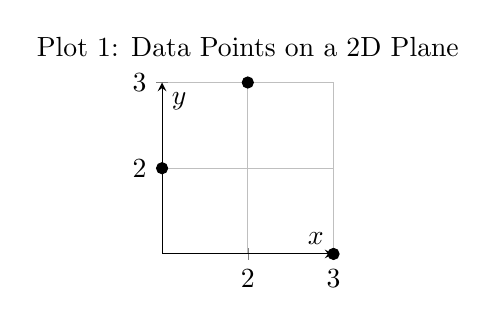
\begin{tikzpicture}
            \begin{axis}[
                title={Plot 1: Data Points on a 2D Plane},
                xlabel={$x$},
                ylabel={$y$},
                axis lines=middle,
                grid=major,
                width=0.31\textwidth,
                height=0.31\textwidth,
                xtick={1, 2, 3},
                ytick={0, 1, 2, 3}
            ]
                \addplot[only marks, mark=*, mark size=2pt] coordinates {(1,2) (2,3) (3,1)};
            \end{axis}
        \end{tikzpicture}
        \hspace{1cm}
        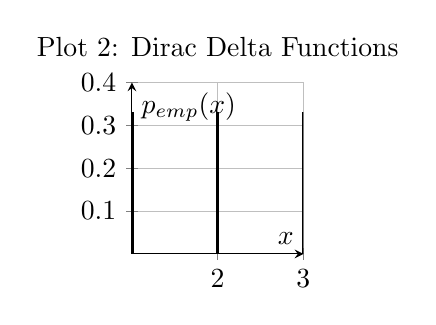
\begin{tikzpicture}
            \begin{axis}[
                title={Plot 2: Dirac Delta Functions},
                xlabel={$x$},
                ylabel={$p_{\text{emp}}(x)$},
                axis lines=middle,
                grid=major,
                width=0.31\textwidth,
                height=0.31\textwidth,
                ymin=0, ymax=0.4,
                xtick={1,2,3},
                ytick={0,0.1,0.2,0.3,0.4}
            ]
                \addplot[very thick] coordinates {(1,0) (1,0.33)};
                \addplot[very thick] coordinates {(2,0) (2,0.33)};
                \addplot[very thick] coordinates {(3,0) (3,0.33)};
            \end{axis}
        \end{tikzpicture}
        \hspace{1cm}
        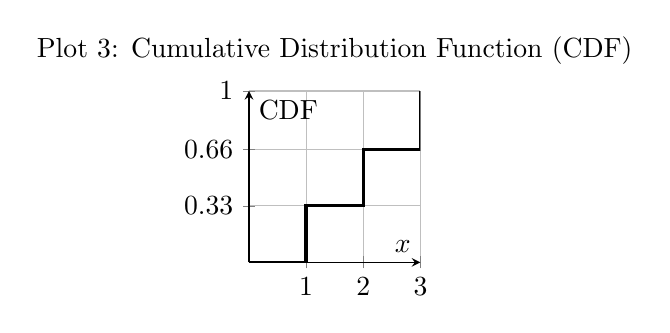
\begin{tikzpicture}
            \begin{axis}[
                title={Plot 3: Cumulative Distribution Function (CDF)},
                xlabel={$x$},
                ylabel={CDF},
                axis lines=middle,
                grid=major,
                width=0.31\textwidth,
                height=0.31\textwidth,
                ymin=0, ymax=1,
                xtick={1, 2, 3},
                ytick={0, 0.33, 0.66, 1}
            ]
                \addplot[very thick] coordinates {(0,0) (1,0) (1,0.33) (2,0.33) (2,0.66) (3,0.66) (3,1)};
            \end{axis}
        \end{tikzpicture}
    \end{center}
    
\end{intuitbox}

\marginnote[-120pt]{    \refsb{Recommended Viewing}{
  \href{https://www.youtube.com/watch?v=7f3YFT7bsmg}{Lecture on Empirical Distribution}\smallskip

  Empirical Statistics: When you compute statistics from a dataset, you're really computing statistics for its empirical distribution.\smallskip

  A dataset is, in essence, a distribution.
}}


\textbf{Empirical Distribution:} Suppose we have a set of data samples 

$$D = \{x^{(1)}, x^{(2)}, \ldots, x^{(N)}\} $$

derived from a random variable \(X\). We can approximate the distribution of \(X\) using a set of delta functions on these samples:
% Represents the distribution of a given data set \(D = \{x^{(1)}, \ldots, x^{(N)}\}\).
\begin{itemize}
    \item For a given data set \(D\), the empirical distribution \(p_{\text{emp}}(x)\) is defined as:
    \[
    p_{\text{emp}}(x) := \frac{1}{N} \sum_{i=1}^N \delta_{x_i}(x)
    \]
    where \(\delta_{x_i}(x)\) is the Dirac measure centred at \(x_i\).
    \item \textbf{Dirac Measure:} \(\delta_{x_i}(x)\) is a function that is 1 if \(x = x_i\) and 0 otherwise. Formally, it is defined as:
    \[
    \delta_{x_i}(x) = \begin{cases} 
    1, & \text{if } x = x_i \\
    0, & \text{if } x \neq x_i 
    \end{cases}
    \]
    \item Explanation: The empirical distribution assigns equal probability \( \frac{1}{N} \) to each observed data point \(x_i\). It is a discrete distribution that places mass only on the observed data points.
    \item In general, one can associate weights with each element of the empirical distribution, i.e., \(p_{\text{emp}}(x) = \frac{1}{N} \sum_{i=1}^N w_i \delta_{x_i}(x)\) as long as each \( 0 \leq w_i \leq 1 \) and \( \sum_{i=1}^N w_i = 1 \).
\end{itemize}

\section{Continuous Random Variables}

\subsection{Gaussian (Normal) Distribution}
\textbf{Probability Density Function (p.d.f):}
\begin{itemize}
    \item Formula: \[
    N(x \mid \mu, \sigma^2) = \frac{1}{\sqrt{2\pi\sigma^2}} \exp\left(-\frac{(x - \mu)^2}{2\sigma^2}\right)
    \]
    \item Mean: \(\mu = \mathbb{E}[X]\).
    \item Variance: \(\sigma^2 = \text{Var}[X]\).
    \item Standard Normal Distribution: \(X \sim N(0, 1)\).
    \item Precision: \(\lambda = \frac{1}{\sigma^2}\).
\end{itemize}
\textbf{Cumulative Distribution Function (CDF):}
\begin{itemize}
    \item Formula: \[
    \Phi(x; \mu, \sigma^2) = \int_{-\infty}^x N(z; \mu, \sigma^2) \, dz
    \]
    \item In terms of the error function (erf):
        \[
        \Phi(x; \mu, \sigma^2) = \frac{1}{2} \left[1 + \text{erf}\left(\frac{z}{\sqrt{2}}\right)\right]
        \]
        where \(z = \frac{x - \mu}{\sigma}\) and
        \[
        \text{erf}(x) = \frac{1}{\sqrt{\pi}} \int_0^x \exp(-t^2) \, dt
        \]
\end{itemize}


\section{Viewing Data}

\begin{itemize}
    \item Data (coordinates) Perspective (Design Matrix) 
    \item Set Perspective
    \begin{itemize}
        \item Combination invariant
        \item Allows for natural language....??
    \end{itemize}
    \item Empirical Distribution Perspective
    \begin{itemize}
        \item i.i.d
    \end{itemize}
\end{itemize}


\section{Example Scene: Self-Driving Car}
\sn{Notation and Gotchas}{
    The lecture use $x_i$ to denote the $i$-th feature, and $x^{(i)}$ to denote the $i$-th data point. The slides however seem to denote $x_i$ as the $i$-th data point. The notes follow the former convention.\\

    Also, it is generally assumed that in a classification problem, the classes are distinct and mutually exclusive, so an image is either a dog or a cat (multi-class classfication) but not a combination of both (multi-label classification). The course focuses on the former convention.

}
Take a case of the self-driving car. There are several facets:
\begin{enumerate}
    \item \textbf{Object Recognition: }identifying objects in the scene (classification)
          \begin{itemize}[noitemsep]
              \item An image is a 2D array of pixel values. For a colour image, each pixel has 3 values (RGB).
              \item \textbf{Input:}
                    \begin{equation}
                        x \in \mathbb{R}^{H \times W \times C}
                    \end{equation}
                    where $H$ is height, $W$ is width, and $C$ is the number of channels (e.g. 3 for RGB)
              \item \textbf{Output:} We would like to detect if something is a background, another vehicle, the ground level, or a pedestrian. Let's say there are $m$ outcomes, making this a \textbf{classification problem}. Naively, let
                    $y \in \mathbb{R}^m$. However, these numbers are just arbitrary i.e. raw scores. It would make more sense to refine the output to a probability distribution over the $m$ classes: \\
                    \begin{equation}
                        y \in \Delta^m \quad \text{where }\sum_{i=1}^{m} y_i = 1
                    \end{equation}
                    Where the $\Delta^m$ is the $m$-simplex, where the sum of all elements is 1. This provides a measure of ``confidence'' in the prediction. Example: To choose between four classes: [Vehicle, Pedestrian, Road, Background], the output could be $[0.1, 0.7, 0.1, 0.1]$. This means the model is 70\% confident that the object is a pedestrian.
              \item \textbf{Our objective is to learn a function:}
                    \begin{equation}
                        f^\theta : x^{(i)} \mapsto y^{(i)} \quad \text{where } \theta \text{ are model parameters}, x^{(i)} \in \mathbb{R}^{H \times W \times C}, y^{(i)} \in \Delta^m
                    \end{equation}
                    \begin{marginfigure}
                        \centering
                        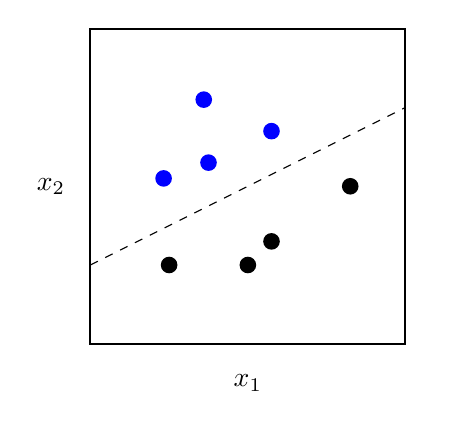
\begin{tikzpicture}
                            % Draw the outer square
                            \draw[thick, black] (0,0) rectangle (4,4);
                            % Draw the blue points
                            \fill[blue] (1.44,3.1) circle (3pt);
                            \fill[blue] (1.5,2.3) circle (3pt);
                            \fill[blue] (0.93,2.1) circle (3pt);
                            \fill[blue] (2.3,2.7) circle (3pt);
                            % Draw the black points
                            \fill[black] (3.3,2) circle (3pt);
                            \fill[black] (2.3,1.3) circle (3pt);
                            \fill[black] (2,1) circle (3pt);
                            \fill[black] (1,1) circle (3pt);
                            % Labels for the axes
                            \node at (2,-0.5) {$x_1$};
                            \node at (-0.5,2) {$x_2$};
                            % Dashed separator
                            \draw[dashed] (0,1)--(4,3) node[right] {};
                        \end{tikzpicture}
                        \caption{Simplified example for $f^\theta$}
                        \label{fig:1_classification}
                    \end{marginfigure}
                    A simplified example for $f^\theta$ is shown in Figure \ref{fig:1_classification}. Ideally, we want a separator that separates the input space into $m$ distinct regions according to observed data.

              \item \textbf{Data Formalisation (1): }We can view our dataset as a set of $N$ pairs where $x^{(i)}$ is an image and $y^{(i)}$ is the corresponding label. More neatly put,
                    \begin{equation}
                        \mathcal{D} = \{(x^{(i)}, y^{(i)})\}_{i=1}^{N}, \quad x^{(i)} \in \mathbb{R}^{H \times W \times C}, y^{(i)} \in \Delta^m
                    \end{equation}
              \item \textbf{Data Formalisation (2): } We could also view the dataset as an empirical distribution over the data space like in Figure \ref{fig:1_distribution}:
                    \begin{equation}
                        \mathcal{D} = \{x^{(i)}, y^{(i)}\}_{i=1}^{N} \sim p_{\text{data}}(x, y)
                    \end{equation}
                    \begin{marginfigure}
                        \centering
                        \begin{tikzpicture}
                            \begin{axis}[
                                view={0}{90},
                                axis on top,
                                enlargelimits=false,
                                colormap/viridis,
                                xlabel={$x_1$},
                                ylabel={$x_2$},
                                % colorbar,
                                samples=50, % Adjusting the sample size
                                domain=-5:5,
                                width=2in,
                                height=2in
                            ]
                            
                            % First contour group
                            \addplot3[
                                contour gnuplot={
                                    levels={0.25, 0.4, 0.55, 0.65, 0.79, 1, 1.25, 1.5}
                                }
                            ]
                            {exp(-((x)^2 + (1.4*y)^2))};
                    
                            % Second contour group
                            \addplot3[
                                contour gnuplot={
                                    levels={0.25, 0.4, 0.55, 0.65, 0.79, 1, 1.25, 1.5}
                                }
                            ]
                            {exp(-((2*x+2)^2 + (y+2)^2))};
                            
                            \end{axis}
                        \end{tikzpicture}
                        \caption{Viewing the dataset as an empirical distribution}
                        \label{fig:1_distribution}
                    \end{marginfigure}
                    



          \end{itemize}
          \item \textbf{Route Planning:} 
          We aim to predict the optimal path, where the prediction function \( f^\theta \) takes spatial data and environmental conditions as input and outputs a route (either as a series of decisions or waypoints).
          \begin{itemize}[noitemsep]
              \item \textbf{Input:}
              \begin{equation}
                  x \in \mathbb{R}^{n}
              \end{equation}
              where \( x \) could represent a vector of features including road conditions, traffic density, and start/end coordinates.
              
              \item \textbf{Output:} 
              A route \( y \), represented either as a classification over a set of discrete routes, or as continuous waypoints:
              \begin{equation}
                  f^\theta : x \mapsto y
              \end{equation}
              Here, \( y \in \mathbb{R}^m \) for \( m \) possible waypoints (or classes, if we use a discrete route classification).
          \end{itemize}
          The objective is to minimise the difference between predicted and actual routes, defined as a suitable loss function \( \mathcal{L}(f^\theta(x), y) \).

    \item \textbf{Speed Control:} 
    \sn{Ordinal Regression here?}{To update}
          In this problem, we predict the optimal driving speed, and \( f^\theta \) models the relationship between environmental and driving conditions and speed.
          \begin{itemize}[noitemsep]
              \item \textbf{Input:} 
              \begin{equation}
                  x \in \mathbb{R}^p
              \end{equation}
              where \( x \) represents features such as current speed, distance to obstacles, road surface, and weather conditions.
              
              \item \textbf{Output:} 
              A continuous speed value \( y \in \mathbb{R} \):
              \begin{equation}
                  f^\theta : x \mapsto y
              \end{equation}
              where \( y \) is the predicted speed. This is a regression problem, so the goal is to minimise the squared error:
              \begin{equation}
                  \mathcal{L}(\theta) = \frac{1}{N} \sum_{i=1}^{N} (f^\theta(x^{(i)}) - y^{(i)})^2
              \end{equation}
          \end{itemize}

    \item \textbf{Steering Angle Prediction:}
          Steering angle prediction aims to output a continuous angle based on the driving conditions, making it a regression problem.
          \begin{itemize}[noitemsep]
              \item \textbf{Input:}
              \begin{equation}
                  x \in \mathbb{R}^q
              \end{equation}
              where \( x \) could represent lane position, vehicle surroundings, and road curvature.
              
              \item \textbf{Output:} 
              The predicted steering angle \( y \in \mathbb{R} \):
              \begin{equation}
                  f^\theta : x \mapsto y
              \end{equation}
              This is also a regression task, and the loss function could again be the squared error:
              \begin{equation}
                  \mathcal{L}(\theta) = \frac{1}{N} \sum_{i=1}^{N} (f^\theta(x^{(i)}) - y^{(i)})^2
              \end{equation}
          \end{itemize}
\end{enumerate}

\section{Mathematics of Linear Models}

Linear models are fundamental in statistics and supervised machine learning. They can:
\begin{itemize}[noitemsep]
    \item Handle linear relationships.
    \item Be augmented with kernels or basis functions to model non-linear relationships.
    \item Provide analytical tractability for studying concepts like convergence, probabilistic modelling, and overfitting.
\end{itemize}
This section introduces the linear regression model.

\subsection{Linear Regression Model}

Linear regression involves performing regression with a linear model in a supervised setting. Given a dataset \(\mathcal{D}\) consisting of input-output pairs \((\bm{x}^{(i)}, y^{(i)})\) for \(i = 1, \ldots, N\):
\begin{itemize}[noitemsep]
    \item \(\bm{x} \in \mathbb{R}^n\) represents the input features.
    \item \(y \in \mathbb{R}\) represents the output or target variable.
    \item Assume a domain \(\mathbb{R}^n\) and a one-dimensional co-domain.
    \item Model: \(f(\bm{x}) = \bm{x}^\top \bm{\theta}\).
    \item Noise: \(\epsilon \sim \mathcal{N}(0, \sigma^2)\).
\end{itemize}
The full model is:
\[
\hat{y}^{(i)} = \bm{x}^{(i)\top} \bm{\theta} + \epsilon
\]

The objective is to find \(\bm{\theta}\) such that \(\hat{y}^{(i)} \approx y^{(i)}\). In other words, we want to find a set of parameters \(\bm{\theta}\) that best explains the relationship between the input features \(\bm{x}\) and the target variable \(y\). This means minimising the difference between the predicted values \(\hat{y}\) and the actual values \(y\).\bigskip

\textbf{Conventions and Notations:}
\begin{itemize}[noitemsep]
    \item Vectors \(\bm{x} \in \mathbb{R}^n\) are column vectors, written as \(n \times 1\) matrices.
    \item \(\bm{x}^\top\) (x transpose) swaps rows and columns of \(\bm{x}\), resulting in a \(1 \times n\) row vector.
\end{itemize}




\begin{referencebox}{Lecture Reading}
    Chapter 1-2 of Kevin Murphy's \textit{Machine Learning: A Probabilistic Perspective}. Chapter 1.4 was not covered, but may be of interest
\end{referencebox}




